\newcommand{\dieuwke}[1]{\textcolor{green!60!black}{DH: #1}}
\newcommand{\lovish}[1]{\textcolor{green!60!black}{LM: #1}}
\newcommand{\TBD}[1]{\textcolor{red!80!black}{\textbf{TBD:} #1}}

\subsection{Pre-trained Language Model}\label{results:pretrained_lm}

In this section, we report evaluation results for our pre-trained \llamathree (Section~\ref{section:pretraining}), comparing with various other models of comparable sizes.
We reproduce results of competitor models whenever possible.
For non-Llama models, we report the best score across results that are publicly reported or (where possible) that we reproduced ourselves.
The specifics of these evaluations, including configurations such as the number of shots, metrics, and other pertinent hyperparameters and settings, can be accessed on our \href{https://github.com/meta-llama/llama-models/blob/main/models/llama3_1/eval_details.md}{Github repository here.} Additionally, we are releasing the data generated as part of evaluations with publicly available benchmarks which can be found on \href{https://huggingface.co/meta-llama}{Huggingface here}.
We evaluate the quality of our models on standard benchmarks (Section~\ref{subsec:automatic_benchmarks}), for robustness to changes in multiple-choice question setups (Section~\ref{subsec:robustness}), and on adversarial evaluations (Section~\ref{subsec:adversarial}). 
We also conduct a contamination analysis to estimate the extent to which our evaluations are impacted by contamination of training data (Section~\ref{subsec:contamination_analysis}).

\subsubsection{Standard Benchmarks}
\label{subsec:automatic_benchmarks}

\begin{table}
    \centering
    \subsection{Speed and Memory Benchmarks}
\label{sec:exp:benchmark}


We benchmark the speed of the SSM scan operation (state expansion $N=16$), as well as the end-to-end
inference throughput of Mamba, in \cref{fig:scan_benchmark}.
Our efficient SSM scan is faster than the best attention implementation that we know of
(FlashAttention-2~\citep{dao2023flashattention2}) beyond sequence length 2K,
and up to 20-40$\times$ faster than a standard scan implementation in
PyTorch.
Mamba achieves 4-5$\times$ higher inference throughput than a Transformer of similar
size, since without the KV cache it can use much higher batch sizes.
For example, a Mamba-6.9B (untrained) would have higher inference throughput than a
$5\times$ smaller Transformer-1.3B.
Details in \cref{sec:exp-details:benchmark}, which additionally includes a benchmark of memory consumption.

    \caption{\textbf{Pre-training benchmarks by category.} Overview of all benchmarks we use to evaluate pre-trained \llamathree models, grouped by capability category.} %
    \label{table:pretraining_benchmarks}
\end{table}

To compare our models with the current state-of-the-art, we evaluate \llamathree on a large number of standard benchmark evaluations shown in Table~\ref{table:pretraining_benchmarks}.
These evaluations cover eight top-level categories: \textbf{(1)} commonsense reasoning; \textbf{(2)} knowledge; \textbf{(3)} reading comprehension; \textbf{(4)} math, reasoning, and problem solving; \textbf{(5)} long context; \textbf{(6)} code; \textbf{(7)} adversarial evaluations; and \textbf{(8)} aggregate evaluations.

\textbf{Experimental setup.}
For each benchmark, we compute scores for \llamathree as well as various other pre-trained models of comparable sizes.
Where possible, we recompute numbers with our own pipeline for other models.
To ensure a fair comparison, we then select the best score between the score that we computed and the reported number for that model with comparable or more conservative settings.
You can find additional details on our evaluation setup \href{https://github.com/meta-llama/llama-models/blob/main/models/llama3_1/eval_details.md}{here}.
For some models, it is not possible to (re)compute benchmark values, for instance, because the pre-trained model is not released or because the API does not provide access to log-probabilities. 
In particular, this is true for all models comparable to \llamathree 405B.
Thus, we do not report category averages for \llamathree 405B, which requires that all numbers are available for all benchmarks.

\textbf{Significance estimates.}
Benchmark scores are estimates of a model's true performance.
These estimates have variance because benchmark sets are finite samples drawn from some underlying distribution.
We follow \citet{madaan2024quantifying} and report on this variance via 95\% confidence intervals (CIs), assuming that benchmark scores are Gaussian distributed.
While this assumption is incorrect (\emph{e.g.}, benchmark scores are bounded), preliminary bootstrap experiments suggest CIs (for discrete metrics) are a good approximation:
$$CI(S) = 1.96 \times \sqrt{\frac{S \times (1 - S)}{N}}.$$
Herein, $S$ is the observed benchmark score (\emph{e.g.}, accuracy or EM) and $N$ the sample size of the benchmark.
We omit CIs for benchmark scores that are not simple averages.
We note that because subsampling is not the only source of variation, our CI values lower bound the actual variation in the capability estimate.

\begin{figure}[t]
    \centering
    \begin{minipage}{.48\textwidth}
    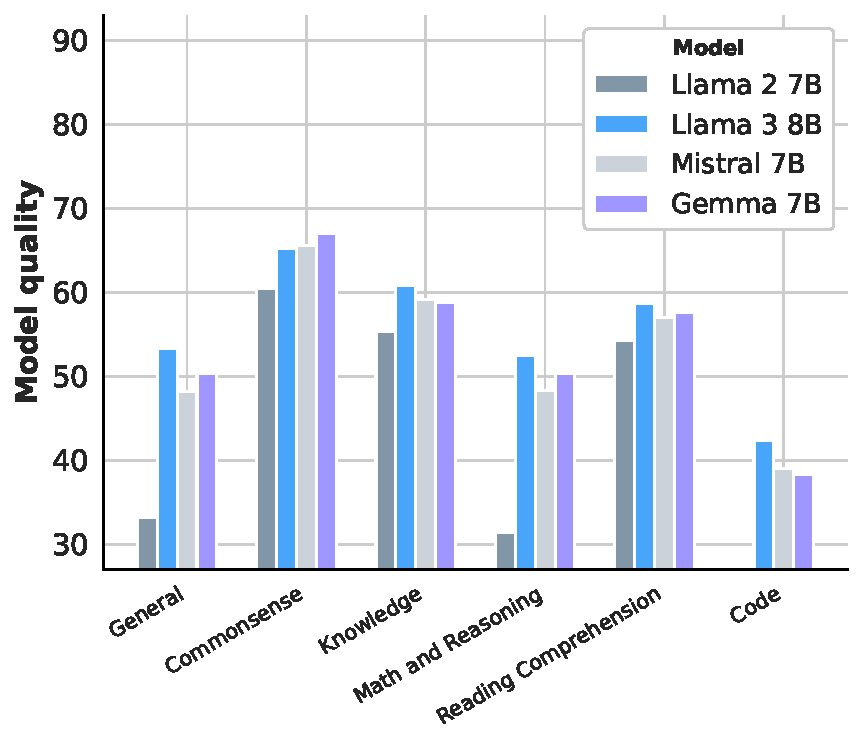
\includegraphics[width=\textwidth]{assets/pretraining_results/aggregate_benchmark_results_8b.pdf}
    \end{minipage}\hfill
    \begin{minipage}{.48\textwidth}
    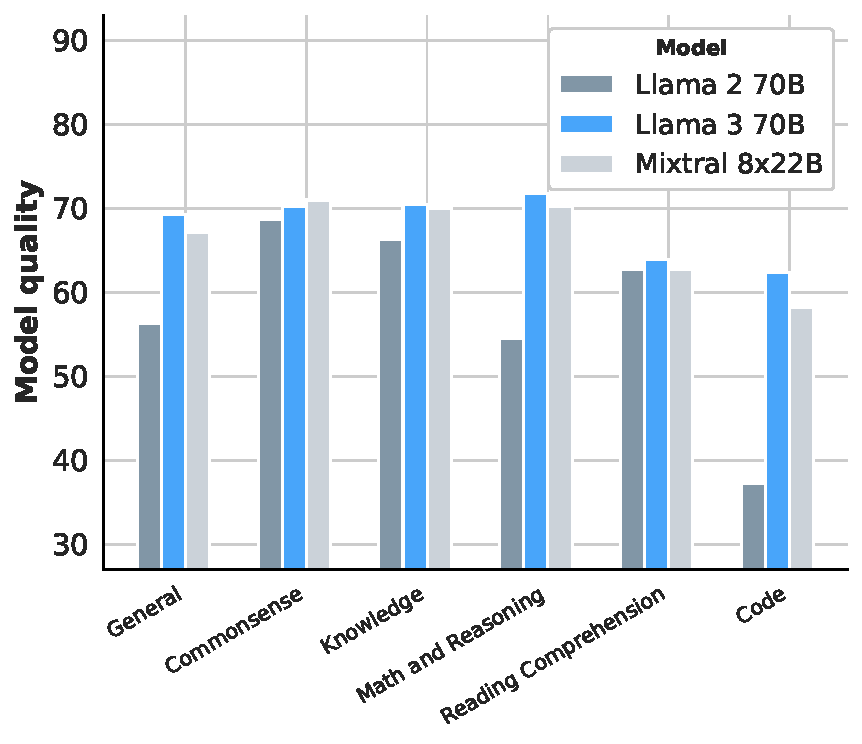
\includegraphics[width=\textwidth]{assets/pretraining_results/aggregate_benchmark_results_70b.pdf}
     \end{minipage}
    \caption{\textbf{Performance of pre-trained \llamathree 8B and 70B models on pre-training benchmarks.} Results are aggregated by capability category by averaging accuracies across all benchmarks corresponding to that category.}
    \label{figure:main_results_pretraining}
\end{figure}


\textbf{Results for 8B and 70B models.} 
Figure~\ref{figure:main_results_pretraining} reports the average performance of \llamathree 8B and 70B on the commonsense reasoning, knowledge, reading comprehension, math and reasoning, and code benchmarks.
The results show that \llamathree 8B outperforms competing models in virtually every category, both in terms of per-category win rate and in terms of average per-category performance.
We also find that \llamathree 70B outperforms its predecessor \llamatwo 70B by a large margin on most benchmarks, with the exception of commonsense benchmarks that are likely saturated.
\llamathree 70B also outperforms Mixtral 8x22B.

\textbf{Detailed results for all models.} 
Table~\ref{table:full_results_pretraining_reading_comprehension}, \ref{table:full_results_code}, \ref{table:full_results_pretraining_commonsense}, \ref{table:full_results_math_reasoning}, \ref{table:full_results_general}, and \ref{table:lc_base_model_evals} present the benchmark performance of pre-trained \llamathree 8B, 70B, and 405B models on reading comprehension tasks, coding tasks, commonsense understanding tasks, mathematical reasoning tasks, and general tasks.
The tables compare Llama 3's performance with that of models of similar size.
The results show that \llamathree 405B performs competitively with other models in its class. 
In particular, \llamathree 405B substantially outperforms prior open-source models.
For long-context, we present more comprehensive results (including probing tasks like needle-in-a-haystack) in Section~\ref{section:results_finetuned}.




\begin{table}
    \centering
    \begin{minipage}{.48\textwidth}
    \begin{NiceTabular}{lccc}
	\CodeBefore
	\Body
	\toprule
	& \multicolumn{3}{c}{\textbf{Reading Comprehension}} \\
	\midrule
	& SQuAD & QuAC & RACE\\
\cmidrule{2-4}
	Llama 3 8B & 77.0 \scriptsize{$\pm$0.8}& \textbf{44.9 \scriptsize{$\pm$1.1}}& \textbf{54.3 \scriptsize{$\pm$1.4}} \\
	Mistral 7B &73.2 \scriptsize{$\pm$0.8}& 44.7 \scriptsize{$\pm$1.1}& 53.0 \scriptsize{$\pm$1.4} \\
	Gemma 7B &\textbf{81.8 \scriptsize{$\pm$0.7}}& 42.4 \scriptsize{$\pm$1.1}& 48.8 \scriptsize{$\pm$1.4} \\
	\cmidrule{2-4}
	Llama 3 70B & 81.8 \scriptsize{$\pm$0.7}& \textbf{51.1 \scriptsize{$\pm$1.1}}& 59.0 \scriptsize{$\pm$1.4} \\
	Mixtral 8$\times$22B &\textbf{84.1 \scriptsize{$\pm$0.7}}& 44.9 \scriptsize{$\pm$1.1}& \textbf{59.2 \scriptsize{$\pm$1.4}} \\
	\cmidrule{2-4}
	Llama 3 405B & \textbf{81.8 \scriptsize{$\pm$0.7}}& \textbf{53.6 \scriptsize{$\pm$1.1}}& \textbf{58.1 \scriptsize{$\pm$1.4}} \\
	GPT-4 & -- & -- & -- \\
	Nemotron 4 340B &--& --& -- \\
	Gemini Ultra &--& -- & -- \\
	\bottomrule
\end{NiceTabular}

    \caption{\textbf{Pre-trained model performance on reading comprehension tasks.} Results include 95\% confidence intervals.}
    \label{table:full_results_pretraining_reading_comprehension}
    \end{minipage}\hfill
    \begin{minipage}{.48\textwidth}
    \centering
    \begin{NiceTabular}{lcc}
	\CodeBefore
	\Body
	\toprule
	& \multicolumn{2}{c}{\textbf{Code}} \\
	\midrule
	& HumanEval & MBPP\\
\cmidrule{2-3}
	Llama 3 8B & \textbf{37.2 \scriptsize{$\pm$7.4}}& \textbf{47.6 \scriptsize{$\pm$4.4}} \\
	Mistral 7B &30.5 \scriptsize{$\pm$7.0}& 47.5 \scriptsize{$\pm$4.4} \\
	Gemma 7B &32.3 \scriptsize{$\pm$7.2}& 44.4 \scriptsize{$\pm$4.4} \\
	\cmidrule{2-3}
	Llama 3 70B & \textbf{58.5 \scriptsize{$\pm$7.5}}& 66.2 \scriptsize{$\pm$4.1} \\
	Mixtral 8$\times$22B &45.1 \scriptsize{$\pm$7.6}& \textbf{71.2 \scriptsize{$\pm$4.0}} \\
	\cmidrule{2-3}
	Llama 3 405B & 61.0 \scriptsize{$\pm$7.5}& \textbf{73.4 \scriptsize{$\pm$3.9}} \\
	GPT-4 &67.0 \scriptsize{$\pm$7.2}& -- \\
	Nemotron 4 340B &57.3 \scriptsize{$\pm$7.6}& -- \\
	Gemini Ultra &\textbf{74.4 \scriptsize{$\pm$6.7}}& -- \\
	\bottomrule
\end{NiceTabular}

    \caption{\textbf{Pre-trained model performance on coding tasks.} Results include 95\% confidence intervals.}
    \label{table:full_results_code}
    \end{minipage}
\end{table}

\begin{table}
\centering
\begin{NiceTabular}{lccccc}
	\CodeBefore
	\Body
	\toprule
	& \multicolumn{5}{c}{\textbf{Commonsense Understanding}} \\
	\midrule
	& CommonSenseQA & PiQA & SiQA & OpenBookQA & Winogrande\\
\cmidrule{2-6}
	Llama 3 8B & \textbf{75.0 \scriptsize{$\pm$2.5}}& 81.0 \scriptsize{$\pm$1.8}& 49.5 \scriptsize{$\pm$2.2}& 45.0 \scriptsize{$\pm$4.4}& 75.7 \scriptsize{$\pm$2.0} \\
	Mistral 7B &71.2 \scriptsize{$\pm$2.6}& \textbf{83.0 \scriptsize{$\pm$1.7}}& 48.2 \scriptsize{$\pm$2.2}& 47.8 \scriptsize{$\pm$4.4}& \textbf{78.1 \scriptsize{$\pm$1.9}} \\
	Gemma 7B &74.4 \scriptsize{$\pm$2.5}& 81.5 \scriptsize{$\pm$1.8}& \textbf{51.8 \scriptsize{$\pm$2.2}}& \textbf{52.8 \scriptsize{$\pm$4.4}}& 74.7 \scriptsize{$\pm$2.0} \\
	\cmidrule{2-6}
	Llama 3 70B & \textbf{84.1 \scriptsize{$\pm$2.1}}& 83.8 \scriptsize{$\pm$1.7}& \textbf{52.2 \scriptsize{$\pm$2.2}}& 47.6 \scriptsize{$\pm$4.4}& 83.5 \scriptsize{$\pm$1.7} \\
	Mixtral 8$\times$22B &82.4 \scriptsize{$\pm$2.2}& \textbf{85.5 \scriptsize{$\pm$1.6}}& 51.6 \scriptsize{$\pm$2.2}& \textbf{50.8 \scriptsize{$\pm$4.4}}& \textbf{84.7 \scriptsize{$\pm$1.7}} \\
	\cmidrule{2-6}
	Llama 3 405B & \textbf{85.8 \scriptsize{$\pm$2.0}}& \textbf{85.6 \scriptsize{$\pm$1.6}}& \textbf{53.7 \scriptsize{$\pm$2.2}}& \textbf{49.2 \scriptsize{$\pm$4.4}}& 82.2 \scriptsize{$\pm$1.8} \\
	GPT-4 &--& --& --& --& 87.5 \scriptsize{$\pm$1.5} \\
	Nemotron 4 340B  &--& --& --& --& \textbf{89.5 \scriptsize{$\pm$1.4}} \\
	\bottomrule
\end{NiceTabular}

\caption{\textbf{Pre-trained model performance on commonsense understanding tasks.} Results include 95\% confidence intervals.}
\label{table:full_results_pretraining_commonsense}
\end{table}

\begin{table}
\centering
\begin{NiceTabular}{lccccc}
	\CodeBefore
	\Body
	\toprule
	& \multicolumn{5}{c}{\textbf{Math and Reasoning}} \\
	\midrule
	& GSM8K & MATH & ARC-C & DROP & WorldSense\\
\cmidrule{2-6}
	Llama 3 8B & \textbf{57.2 \scriptsize{$\pm$2.7}}& 20.3 \scriptsize{$\pm$1.1}& \textbf{79.7 \scriptsize{$\pm$2.3}}& \textbf{59.5 \scriptsize{$\pm$1.0}}& 45.5 \scriptsize{$\pm$0.3} \\
	Mistral 7B &52.5 \scriptsize{$\pm$2.7}& 13.1 \scriptsize{$\pm$0.9}& 78.2 \scriptsize{$\pm$2.4}& 53.0 \scriptsize{$\pm$1.0}& 44.9 \scriptsize{$\pm$0.3} \\
	Gemma 7B &46.4 \scriptsize{$\pm$2.7}& \textbf{24.3 \scriptsize{$\pm$1.2}}& 78.6 \scriptsize{$\pm$2.4}& 56.3 \scriptsize{$\pm$1.0}& \textbf{46.0 \scriptsize{$\pm$0.3}} \\
	\cmidrule{2-6}
	Llama 3 70B & 83.7 \scriptsize{$\pm$2.0}& 41.4 \scriptsize{$\pm$1.4}& \textbf{92.9 \scriptsize{$\pm$1.5}}& \textbf{79.6 \scriptsize{$\pm$0.8}}& \textbf{61.1 \scriptsize{$\pm$0.3}} \\
	Mixtral 8$\times$22B &\textbf{88.4 \scriptsize{$\pm$1.7}}& \textbf{41.8 \scriptsize{$\pm$1.4}}& 91.9 \scriptsize{$\pm$1.6}& 77.5 \scriptsize{$\pm$0.8}& 51.5 \scriptsize{$\pm$0.3} \\
	\cmidrule{2-6}
	Llama 3 405B & 89.0 \scriptsize{$\pm$1.7}& \textbf{53.8 \scriptsize{$\pm$1.4}}& 96.1 \scriptsize{$\pm$1.1}& \textbf{84.8 \scriptsize{$\pm$0.7}}& \textbf{63.7 \scriptsize{$\pm$0.3}} \\
	GPT-4 &\textbf{92.0 \scriptsize{$\pm$1.5}}& --& \textbf{96.3 \scriptsize{$\pm$1.1}}& 80.9 \scriptsize{$\pm$0.8}& -- \\
	Nemotron 4 340B  &--& --& 94.3 \scriptsize{$\pm$1.3}& --& -- \\
    Gemini Ultra & ~88.9$^{\diamondsuit}$\scriptsize{$\pm$1.7} & ~53.2\scriptsize{$\pm$1.4}& --& 82.4$^\triangle$ \scriptsize{$\pm$0.8} & -- \\
	\bottomrule
\end{NiceTabular}

\caption{\textbf{Pre-trained model performance on math and reasoning tasks.} Results include 95\% confidence intervals. $^\diamondsuit$11-shot. $^\triangle$Variable shot.}
\label{table:full_results_math_reasoning}
\end{table}

\begin{table}
\centering
    \begin{NiceTabular}{lcccc}
	\CodeBefore
	\Body
	\toprule
	& \multicolumn{4}{c}{\textbf{General}} \\
	\midrule
	& MMLU & MMLU-Pro & AGIEval & BB Hard\\
\cmidrule{2-5}
	Llama 3 8B & \textbf{66.7}& \textbf{37.1}& \textbf{47.8 \scriptsize{$\pm$1.9}}& \textbf{64.2 \scriptsize{$\pm$1.2}} \\
	Mistral 7B &63.6& 32.5 & 42.7 \scriptsize{$\pm$1.9}& 56.8 \scriptsize{$\pm$1.2} \\
	Gemma 7B &64.3& 35.1 & 46.0 \scriptsize{$\pm$1.9}& 57.7 \scriptsize{$\pm$1.2} \\
	\cmidrule{2-5}
	Llama 3 70B & \textbf{79.3}& \textbf{53.8}& \textbf{64.6 \scriptsize{$\pm$1.9}}& \textbf{81.6 \scriptsize{$\pm$0.9}} \\
	Mixtral 8$\times$22B &77.8& 51.5 & 61.5 \scriptsize{$\pm$1.9}& 79.5 \scriptsize{$\pm$1.0} \\
	\cmidrule{2-5}
	Llama 3 405B & 85.2& \textbf{61.6}& \textbf{71.6 \scriptsize{$\pm$1.8}}& \textbf{85.9 \scriptsize{$\pm$0.8}} \\
	GPT-4 &\textbf{86.4}& --& --& -- \\
	Nemotron 4 340B  &81.1& --& --& 85.4 \scriptsize{$\pm$0.9} \\
	Gemini Ultra &83.7& --& --& 83.6 \scriptsize{$\pm$0.9} \\
	\bottomrule
\end{NiceTabular}

    \caption{\textbf{Pre-trained model performance on general language tasks.} Results include 95\% confidence intervals.}
\label{table:full_results_general}
\end{table}



\subsubsection{Model Robustness}\label{subsec:robustness}

In addition to performance on benchmarks, robustness is an important factor in the quality of pre-trained language models.
We investigate the robustness of our pre-trained language models to design choices in multiple-choice question (MCQ) setups.
Prior work has reported that model performance can be sensitive to seemingly arbitrary design choices in such setups, for example, model scores and even rankings may change with the order and labels of the in-context examples \citep[]{lu-etal-2022-fantastically,zhao2021calibrate,robison2023leveraging,liang2022holistic,gupta2024changinganswerorderdecrease}, the exact format of the prompt \citep{weber2023icl,mishra-etal-2022-reframing}, or the answer choice format and order \citep{alzahrani2024when,wang2024beyond,zheng2023large}.
Motivated by this work, we use the MMLU benchmark to evaluate the robustness of our pre-trained models to: \textbf{(1)} few-shot label bias, \textbf{(2)} label variants, \textbf{(3)} answer order, and \textbf{(4)} prompt format:

\begin{figure}[t]
    \centering
    \begin{subfigure}[b]{0.49\textwidth}
        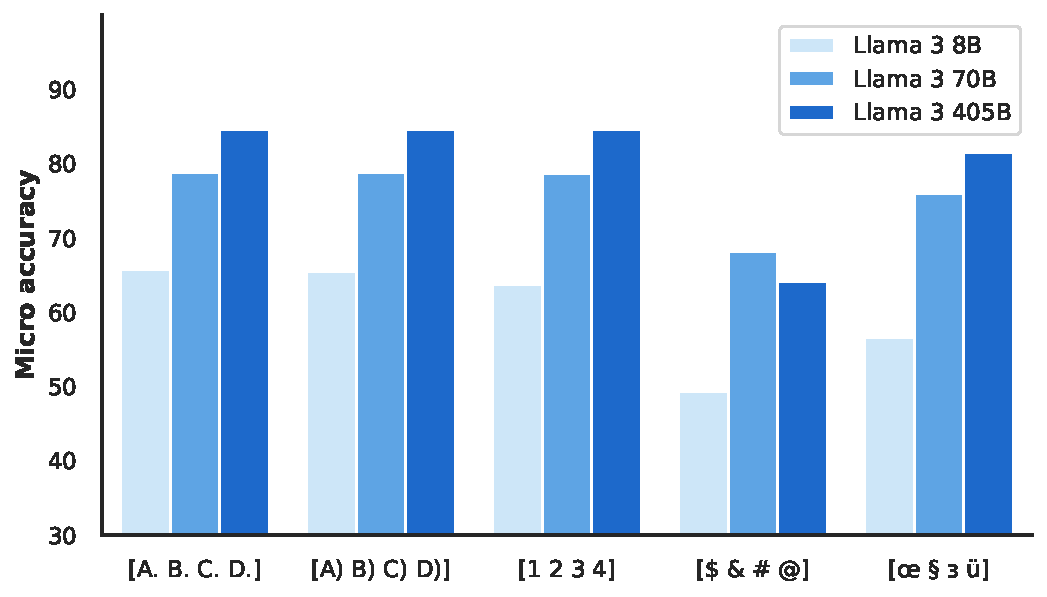
\includegraphics[width=\textwidth]{assets/pretraining_results/mmlu_label_variants.pdf}
        \label{figure:mmlu_label_variants}
    \end{subfigure}
    \hspace{5mm}
    \begin{subfigure}[b]{0.33\textwidth}
        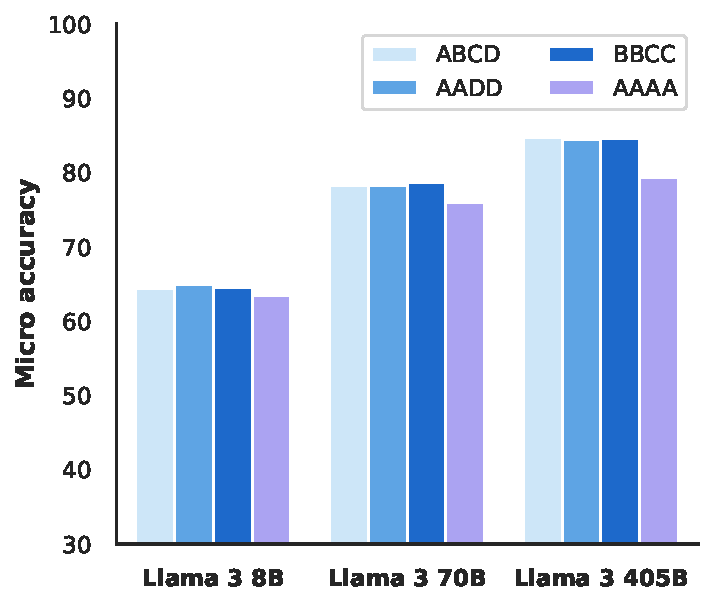
\includegraphics[width=\textwidth]{assets/pretraining_results/fewshot_label_bias_mmlu.pdf}
        \label{figure:fewshot_label_bias_mmlu}
    \end{subfigure}
    \caption{\textbf{Robustness of our pre-trained language models to different design choices in the MMLU benchmark.} \emph{Left:} Performance for different label variants.  \emph{Right:} Performance for different labels present in few-shot examples. }
    \label{figure:robustness1}
\end{figure}

\begin{figure}[t]
    \centering
    \begin{subfigure}[b]{0.47\textwidth}
        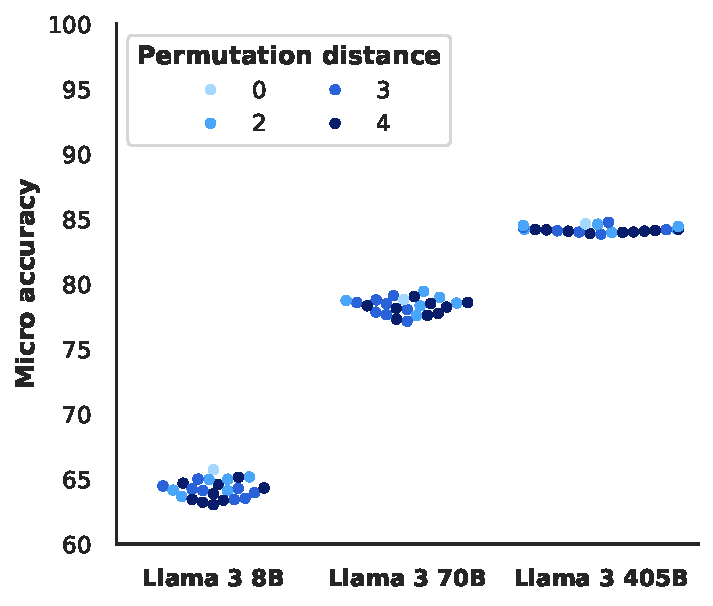
\includegraphics[width=\textwidth]{assets/pretraining_results/permutation_robustness_mmlu_swarm.pdf}
        \label{figure:permutation_robustness_swarm}
    \end{subfigure}
    \begin{subfigure}[b]{0.47\textwidth}
        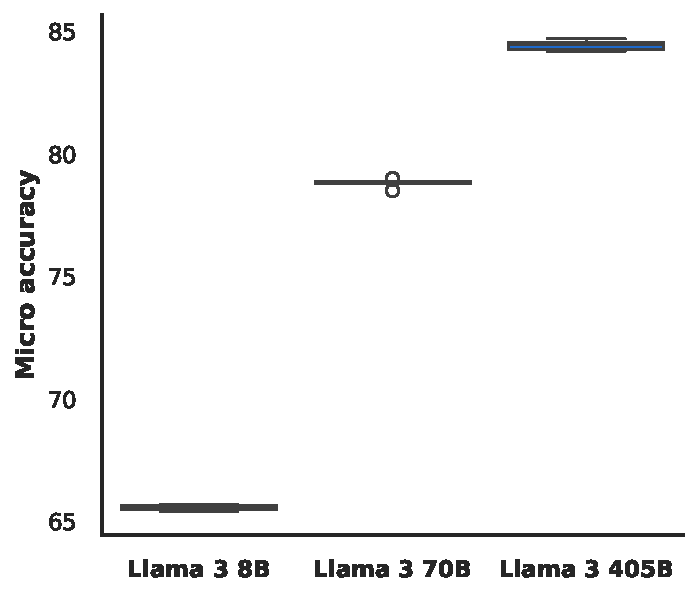
\includegraphics[width=\textwidth]{assets/pretraining_results/paraphrase_robustness_MMLU.pdf}
        \label{figure:mmlu_paraphrases}
    \end{subfigure}
    \caption{\textbf{Robustness of our pre-trained language models to different design choices in the MMLU benchmark.} \emph{Left:} Performance for different answer orders. \emph{Right:} Performance for different prompt formats.}\label{fig:permutation_robustness}
    \label{figure:robustness2}
\end{figure}

\begin{itemize}

\item \textbf{Few-shot label bias.}
Following \citet{zheng2023large} and \citet{weber-etal-2023-mind}, we investigate the impact of the distribution of labels in four-shot examples.
Specifically, we consider settings in which: (1) all few-shot examples have the same label (\texttt{A A A A}); (2) all examples have a different label (\texttt{A B C D}); and (3) there are only two labels present (\texttt{A A B B} and \texttt{C C D D}).

\item \textbf{Label variants.} 
We also study model response to different choice token sets.
We consider the two sets proposed by \citet{alzahrani2024when}: namely, a set of common language independent tokens (\texttt{\$ \& \# @}) and a of rare tokens (\texttt{œ § \foreignlanguage{russian}{з} ü}) that do not have any implicit relative order.
We also consider two versions of the canonical labels (\texttt{A. B. C. D.} and \texttt{A) B) C) D)}) and a numerical list (\texttt{1. 2. 3. 4.}).

\item \textbf{Answer order.}
Following \citet{wang2024beyond}, we compute how stable the results are across different answer orders.
To compute this, we remap all the answers in the dataset according to a fixed permutation.
For example, for the permutation \texttt{A B C D}, all answer options with label \texttt{A} and \texttt{B} keep their label, and all answer options with label \texttt{C} get label \texttt{D}, and vice versa.

\item \textbf{Prompt format.}
We evaluate variance in performance across five task prompts that differ in the level of information provided: one prompt simply asks the model to answer the question, whereas other prompts assert the expertise of the model or that the best answer should be chosen.

\end{itemize}

Figure~\ref{figure:robustness1} presents the results of our experiments studying robustness of model performance to label variants (left) and few-shot label bias (right). 
The results show that our pre-trained language models are very robust to changes in MCQ labels and to the structure of the few-shot prompt labels.
This robustness is particularly pronounced for the 405B parameter model.
Figure~\ref{figure:robustness2} presents the results of our study of robustness to answer order and prompt format.
The results in the figure further underscore the robustness of the performance of our pre-trained language models, in particular, of \llamathree 405B.

\begin{figure}
    \centering
    \begin{subfigure}{0.4\textwidth}
        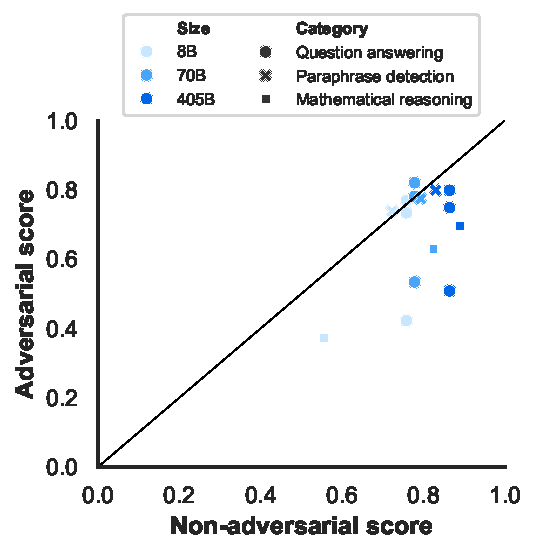
\includegraphics[width=\textwidth]{assets/pretraining_results/adversarial_scores_pretrained}
    \end{subfigure}
    \begin{subfigure}{0.4\textwidth}
        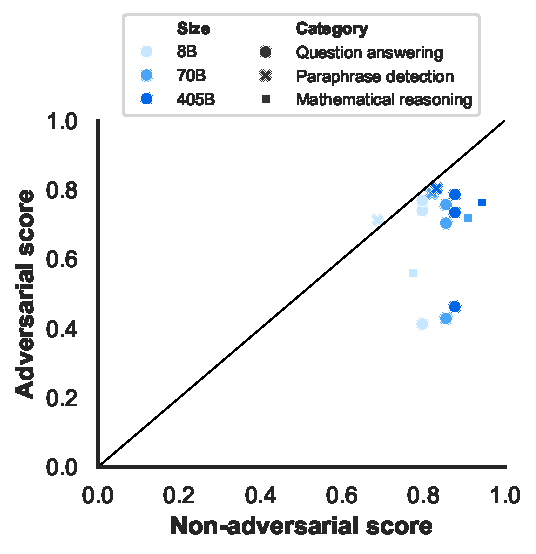
\includegraphics[width=\textwidth]{assets/pretraining_results/adversarial_scores_post_trained}
    \end{subfigure}
    \caption{\textbf{Adversarial versus non-adversarial performance} for question answering, mathematical reasoning, and paraphrase detection benchmarks. \emph{Left:} Results for pre-trained models. \emph{Right:} Results for post-trained models.}\label{fig:pretraining_adversarial}\label{fig:posttraining_adversarial}
\end{figure}

\subsubsection{Adversarial Benchmarks}
\label{subsec:adversarial}

In addition to the benchmarks presented above, we evaluate on several adversarial benchmarks in three areas: question answering, mathematical reasoning, and paraphrase detection.
This testing probes the model's capabilities on tasks specifically created to be challenging and can potentially also point to overfitting on benchmarks.
For question answering, we use Adversarial SQuAD~\citep{jia-liang-2017-adversarial} and Dynabench SQuAD~\citep{kiela-etal-2021-dynabench}.
For mathematical reasoning, we use GSM-Plus \citep{li2024gsm}.
For paraphrase detection, we use PAWS~\citep{zhang-etal-2019-paws}.

Figure~\ref{fig:pretraining_adversarial} presents the scores of \llamathree 8B, 70B, and 405B on the adversarial benchmarks as a function of their performance on non-adversarial benchmarks.
The non-adversarial benchmarks we use are SQuAD~\citep{rajpurkar-etal-2016-squad} for question answering, GSM8K for mathematical reasoning, and QQP~\citep{quoraFirstQuora} for paraphrase detection.
Each datapoint represents a pair of an adversarial and non-adversarial datasets (\emph{e.g.} QQP paired with PAWS), and we show all possible pairs within a category.
The diagonal black line represents parity between adversarial and non-adversarial datasets --- being on the line would indicate the model has similar performance regardless of the adversarial nature.

On paraphrase detection, neither pre-trained nor post-trained models appear to suffer from the type of adversariality with which PAWS was constructed, marking a substantial step with respect to the previous generation of models.
This result confirms the findings of~\citet{weber-etal-2023-mind}, who also found that LLMs are less susceptible to the type of spurious correlations found in several adversarial datasets.
For mathematical reasoning and question answering, however, the adversarial performances are substantially lower than the non-adversarial performances.
This pattern is similar for pre-trained and post-trained models.

\subsubsection{Contamination Analysis}
\label{subsec:contamination_analysis}

We conduct a contamination analysis to estimate to what extent benchmark scores may be influenced by contamination of the evaluation data in the pre-training corpus.
In previous work, several different contamination methods have been used, with various different hyperparameters -- we refer to \citet{singh2024contamination} for an overview.
Any of these methods can suffer from false positives and negatives, and how to best run contamination analyses is currently still an open field of research.
Here, we largely follow the suggestions of \citet{singh2024contamination}.

\begin{wraptable}{r}{0.5\textwidth}
    \centering
    \begin{NiceTabular}{lccc}
    \toprule
    & \multicolumn{3}{c}{\textbf{Llama 3}}\\
    & 8B & 70B & 405B\\ 
    \midrule
    QuALITY {\tiny (5-shot)} & 56.0 \scriptsize{$\pm$2.1} & 82.8 \scriptsize{$\pm$1.6} & 87.6 \scriptsize{$\pm$1.4} \\
    GSM8K {\tiny (16-shot)} & 60.0 \scriptsize{$\pm$9.6} & 83.0 \scriptsize{$\pm$7.4} & 90.0 \scriptsize{$\pm$5.9} \\
    \bottomrule 
    \end{NiceTabular}
    \caption{\textbf{Performance of pre-trained models on long-context tasks.} Results include 95\% confidence intervals.}
    \label{table:lc_base_model_evals}

    \resizebox{0.5\textwidth}{!}{
    \begin{tabular}{lcccc}
    & & & \\  %

        \toprule
        & \textbf{Contam.} & \multicolumn{3}{c}{\textbf{Performance gain est.}}\\
        & & 8B & 70B & 405B \\
        \midrule
        AGIEval & 98 & 8.5 & 19.9 & 16.3 \\
        BIG-Bench Hard & 95 & 26.0 & 36.0 & 41.0 \\
        BoolQ & 96 & 4.0 & 4.7 & 3.9 \\
        CommonSenseQA & 30 & 0.1 & 0.8 & 0.6 \\
        DROP & -- & -- & -- & -- \\
        GSM8K & 41 & 0.0 & 0.1 & 1.3 \\
        HellaSwag & 85 & 14.8 & 14.8 & 14.3 \\
        HumanEval & -- & -- & -- & -- \\
        MATH & 1 & 0.0 & -0.1 & -0.2 \\
        MBPP & -- & -- & -- & -- \\
        MMLU & -- & -- & -- & -- \\
        MMLU-Pro & -- & -- & -- & -- \\
        NaturalQuestions & 52 & 1.6 & 0.9 & 0.8 \\
        OpenBookQA & 21 & 3.0 & 3.3 & 2.6 \\
        PiQA & 55 & 8.5 & 7.9 & 8.1 \\
        QuaC & 99 & 2.4 & 11.0 & 6.4 \\
        RACE & -- & -- & -- & -- \\
        SiQA & 63 & 2.0 & 2.3 & 2.6 \\
        SQuAD & 0 & 0.0 & 0.0 & 0.0 \\
        Winogrande & 6 & -0.1 & -0.1 & -0.2 \\
        WorldSense & 73 & -3.1 & -0.4 & 3.9 \\ %
        \bottomrule
    \end{tabular}
    }
    \caption{\textbf{Percentage of evaluation sets considered to be contaminated} because similar data exists in the training corpus, and the estimated performance gain that may result from that contamination. See the text for details. }
    \label{table:contamination}

\end{wraptable}

\textbf{Method.}
Specifically, \citet{singh2024contamination} propose to select contamination detection methods empirically, based on which method results in the largest difference between the `clean' part of the dataset and the entire dataset, which they call \emph{estimated performance gain}.
For all our evaluation datasets, we score examples based on 8-gram overlap, a method that was found by \citet{singh2024contamination} to be accurate for many datasets.
We consider an example of a dataset $D$ to be contaminated if a ratio $\mathcal{T}_D$ of its tokens are part of an 8-gram occurring at least once in the pre-training corpus.
We select $\mathcal{T}_D$ separately for each dataset, based on which value shows the maximal significant estimated performance gain across the three model sizes.


\textbf{Results.}
In Table~\ref{table:contamination}, we report the percentage of evaluation data that is considered contaminated for the maximal estimated performance gain, as described above, for all key benchmarks.
From the table, we exclude numbers for benchmarks for which the results are not significant, for instance because the clean or contaminated set has too few examples, or because the observed performance gain estimate shows extremely erratic behavior.
In Table \ref{table:contamination}, we observe that for some datasets contamination has a large impact, while for others it does not.
For example, for PiQA and HellaSwag, both the estimation of contamination and the estimation of performance gain are high.
For Natural Questions, on the other hand, the estimated 52\% contamination seems to have virtually no effect on the performance.
For SQuAD and MATH, low thresholds yield high levels of contamination, but no performance gains. This suggests that contamination is either not helpful for these datasets, or that a larger n is required to obtain a better estimate.
Finally, for MBPP, HumanEval, MMLU and MMLU-Pro, other contamination detection methods may be needed: even with higher thresholds, 8-gram overlap gives such high contamination scores that it is impossible to get a good performance gain estimate.




